\documentclass{standalone}
\usepackage{standalone}

\begin{document}
\section{Comparison With Other Tools}
With error free data, NanoMapper works best. It could map exact positions and map only one position where other tools give some worng positions along with the right position. However, when error chunk added in the data, NanoMapper performs well. As mapping to wrong position could be misleading, a penalty should be added for this. It is not possible to check every base is mapped to the right position or not for certain reasons. In fact, tools map overlapped ranges. Considering all of these restrictions, the following equations are used to evaluate the accuracy.
$$\textbf{Right \%} = \frac{\textbf{\# of Base Mapped to Right Range}}{\textbf{Total \# of Mapped Base}}$$
Similarly,
$$\textbf{Wrong \%} = \frac{\textbf{\# of Base Mapped to Out of Right Range}}{\textbf{Total \# of Mapped Base}}$$

With 5\% error chunk added in the synthetic data, the result is like table \ref{tab:error5}.
\begin{table}[]
	\centering
	\caption{Mapping Comparison While 5\% Error Added in Read Data}
	\label{tab:error5}
	\begin{tabular}{|c|c|c|}
		\hline
		\begin{tabular}[c]{@{}c@{}}Name of the\\ Tool\end{tabular} & \begin{tabular}[c]{@{}c@{}}Right Position\\ (\%)\end{tabular} & \begin{tabular}[c]{@{}c@{}}Wrong Position\\ (\%)\end{tabular} \\ \hline
		BWA-MEM & 88.4 & 11.6 \\ \hline
		NanoBLAST & 86.55 & 13.45 \\ \hline
		NanoMapper & 97.42 & 2.58 \\ \hline
	\end{tabular}
\end{table}

\begin{figure}
	\centering
	
	
	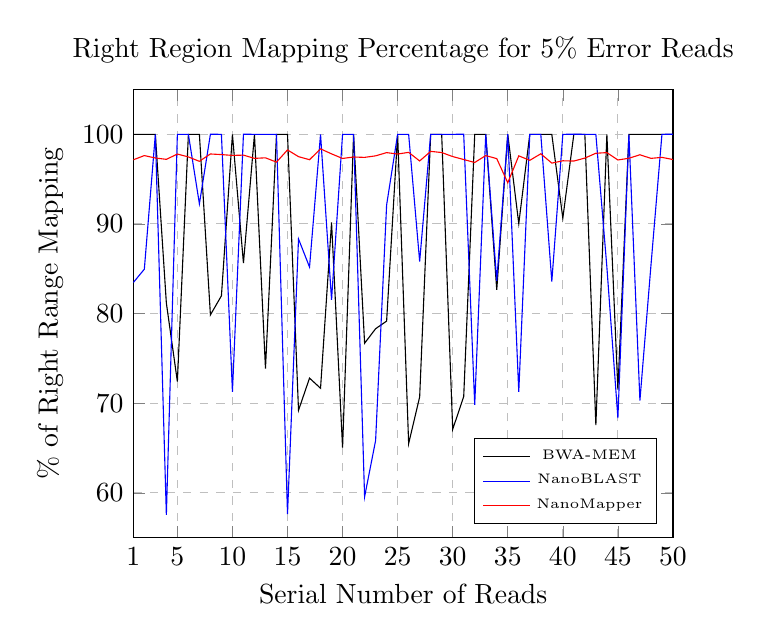
\begin{tikzpicture}
	\begin{axis}[
	title={Right Region Mapping Percentage for 5\% Error Reads},
	xlabel={Serial Number of Reads},
	ylabel={\% of Right Range Mapping  },
	xmin=1, xmax=50,
	ymin=55, ymax=105,
	xtick={1,5,10,15,20,25,30,35,40,45,50},
	ytick={60,70,80,90,100},
	legend pos=south east,
	legend style={font=\tiny},
	ymajorgrids=true,
	xmajorgrids=true,
	grid style=dashed,
	]
	
	\addplot[
	color=black,
	mark=dot,
	]
	coordinates {
		( 1 , 99.98 )( 2 , 99.98 )( 3 , 99.98 )( 4 , 81.17 )( 5 , 72.42 )( 6 , 99.98 )( 7 , 99.98 )( 8 , 79.85 )( 9 , 81.98 )( 10 , 99.98 )( 11 , 85.62 )( 12 , 99.98 )( 13 , 73.86 )( 14 , 99.98 )( 15 , 99.98 )( 16 , 69.21 )( 17 , 72.8 )( 18 , 71.67 )( 19 , 90.16 )( 20 , 65.04 )( 21 , 99.98 )( 22 , 76.69 )( 23 , 78.31 )( 24 , 79.16 )( 25 , 99.98 )( 26 , 65.5 )( 27 , 70.7 )( 28 , 99.98 )( 29 , 99.98 )( 30 , 67.09 )( 31 , 70.74 )( 32 , 99.98 )( 33 , 99.98 )( 34 , 82.64 )( 35 , 99.99 )( 36 , 90.03 )( 37 , 99.99 )( 38 , 99.98 )( 39 , 99.98 )( 40 , 90.64 )( 41 , 99.99 )( 42 , 99.98 )( 43 , 67.56 )( 44 , 99.98 )( 45 , 71.52 )( 46 , 99.98 )( 47 , 99.98 )( 48 , 99.98 )( 49 , 99.98 )( 50 , 99.98 )
	};
	\addlegendentry{BWA-MEM}
	\addplot[
	color=blue,
	mark=dot,
	]
	coordinates {
		( 1 , 83.46 )( 2 , 84.95 )( 3 , 99.99 )( 4 , 57.55 )( 5 , 99.99 )( 6 , 99.99 )( 7 , 92.24 )( 8 , 100.0 )( 9 , 99.99 )( 10 , 71.28 )( 11 , 100.0 )( 12 , 99.99 )( 13 , 99.99 )( 14 , 99.99 )( 15 , 57.63 )( 16 , 88.32 )( 17 , 85.19 )( 18 , 99.99 )( 19 , 81.53 )( 20 , 99.99 )( 21 , 99.99 )( 22 , 59.56 )( 23 , 65.84 )( 24 , 92.11 )( 25 , 99.99 )( 26 , 99.99 )( 27 , 85.81 )( 28 , 99.99 )( 29 , 99.99 )( 30 , 99.99 )( 31 , 100.0 )( 32 , 69.82 )( 33 , 99.99 )( 34 , 83.66 )( 35 , 100.0 )( 36 , 71.27 )( 37 , 99.99 )( 38 , 99.99 )( 39 , 83.58 )( 40 , 99.99 )( 41 , 100.0 )( 42 , 99.99 )( 43 , 99.98 )( 44 , 85.18 )( 45 , 68.35 )( 46 , 99.99 )( 47 , 70.3 )( 48 , 85.34 )( 49 , 99.99 )( 50 , 100.0 )
	};
	\addlegendentry{NanoBLAST}
	\addplot[
	color=red,
	mark=dot,
	]
	coordinates {
		( 1 , 97.15 )( 2 , 97.62 )( 3 , 97.35 )( 4 , 97.2 )( 5 , 97.79 )( 6 , 97.47 )( 7 , 96.98 )( 8 , 97.8 )( 9 , 97.73 )( 10 , 97.64 )( 11 , 97.67 )( 12 , 97.31 )( 13 , 97.37 )( 14 , 96.89 )( 15 , 98.25 )( 16 , 97.5 )( 17 , 97.16 )( 18 , 98.37 )( 19 , 97.81 )( 20 , 97.3 )( 21 , 97.46 )( 22 , 97.42 )( 23 , 97.59 )( 24 , 97.95 )( 25 , 97.79 )( 26 , 97.98 )( 27 , 97.02 )( 28 , 98.09 )( 29 , 97.96 )( 30 , 97.51 )( 31 , 97.18 )( 32 , 96.85 )( 33 , 97.62 )( 34 , 97.28 )( 35 , 94.59 )( 36 , 97.59 )( 37 , 97.09 )( 38 , 97.82 )( 39 , 96.78 )( 40 , 97.04 )( 41 , 97.01 )( 42 , 97.34 )( 43 , 97.88 )( 44 , 97.95 )( 45 , 97.13 )( 46 , 97.32 )( 47 , 97.71 )( 48 , 97.31 )( 49 , 97.42 )( 50 , 97.18 )
	};
	\addlegendentry{NanoMapper}
	\end{axis}
	\end{tikzpicture}
	
	
	\caption{Percentage of Right Range Mapping Comparison Among Tools.} \label{fig:mapComp}
\end{figure}

If we just eliminate mapping length less than or equal to 15, the accuracy reaches 99.17\%. In fact, these should be eliminated as these are not our target K-mer. We are mapping based on long K-mers. However, from figure \ref{fig:mapComp}, it is clear that NanoMapper always maintaining a consistant accuracy where other tools are showing curly curves. The consistent line drift upward when we eliminate K-mers less than or equal to length 15.

\begin{figure}
	\centering
	
	
	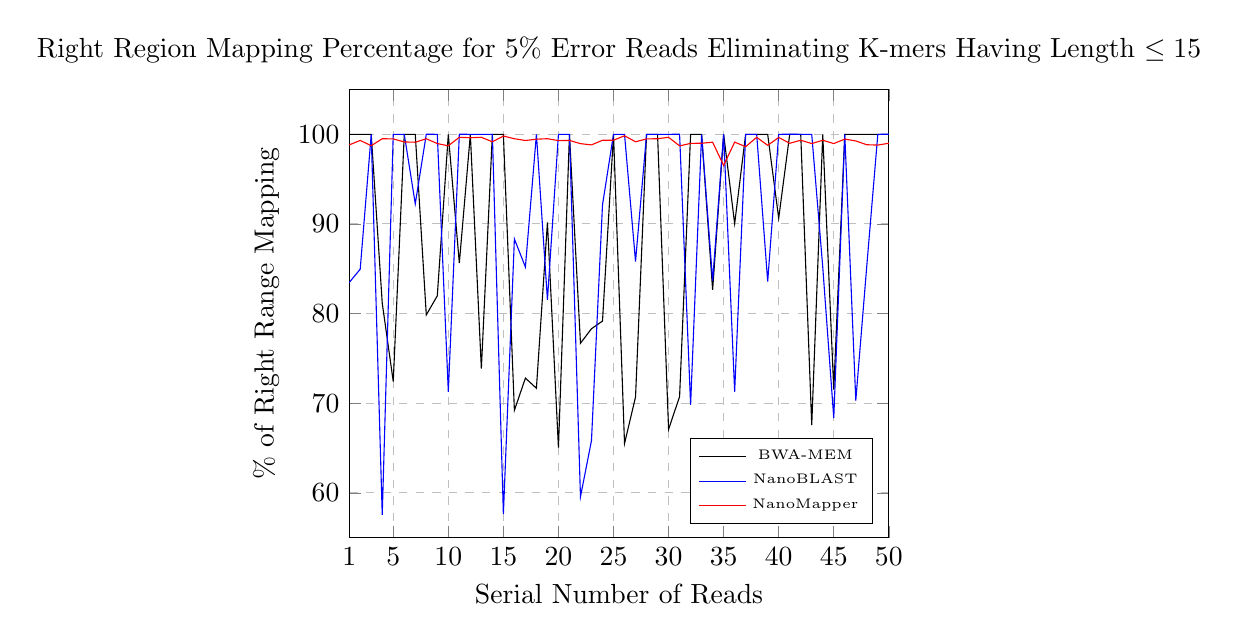
\begin{tikzpicture}
	\begin{axis}[
	title={Right Region Mapping Percentage for 5\% Error Reads Eliminating K-mers Having Length $\leq 15$},
	xlabel={Serial Number of Reads},
	ylabel={\% of Right Range Mapping  },
	xmin=1, xmax=50,
	ymin=55, ymax=105,
	xtick={1,5,10,15,20,25,30,35,40,45,50},
	ytick={60,70,80,90,100},
	legend pos=south east,
	legend style={font=\tiny},
	ymajorgrids=true,
	xmajorgrids=true,
	grid style=dashed,
	]
	
	\addplot[
	color=black,
	mark=dot,
	]
	coordinates {
		( 1 , 99.98 )( 2 , 99.98 )( 3 , 99.98 )( 4 , 81.17 )( 5 , 72.42 )( 6 , 99.98 )( 7 , 99.98 )( 8 , 79.85 )( 9 , 81.98 )( 10 , 99.98 )( 11 , 85.62 )( 12 , 99.98 )( 13 , 73.86 )( 14 , 99.98 )( 15 , 99.98 )( 16 , 69.21 )( 17 , 72.8 )( 18 , 71.67 )( 19 , 90.16 )( 20 , 65.04 )( 21 , 99.98 )( 22 , 76.69 )( 23 , 78.31 )( 24 , 79.16 )( 25 , 99.98 )( 26 , 65.5 )( 27 , 70.7 )( 28 , 99.98 )( 29 , 99.98 )( 30 , 67.09 )( 31 , 70.74 )( 32 , 99.98 )( 33 , 99.98 )( 34 , 82.64 )( 35 , 99.99 )( 36 , 90.03 )( 37 , 99.99 )( 38 , 99.98 )( 39 , 99.98 )( 40 , 90.64 )( 41 , 99.99 )( 42 , 99.98 )( 43 , 67.56 )( 44 , 99.98 )( 45 , 71.52 )( 46 , 99.98 )( 47 , 99.98 )( 48 , 99.98 )( 49 , 99.98 )( 50 , 99.98 )
	};
	\addlegendentry{BWA-MEM}
	\addplot[
	color=blue,
	mark=dot,
	]
	coordinates {
		( 1 , 83.46 )( 2 , 84.95 )( 3 , 99.99 )( 4 , 57.55 )( 5 , 99.99 )( 6 , 99.99 )( 7 , 92.24 )( 8 , 100.0 )( 9 , 99.99 )( 10 , 71.28 )( 11 , 100.0 )( 12 , 99.99 )( 13 , 99.99 )( 14 , 99.99 )( 15 , 57.63 )( 16 , 88.32 )( 17 , 85.19 )( 18 , 99.99 )( 19 , 81.53 )( 20 , 99.99 )( 21 , 99.99 )( 22 , 59.56 )( 23 , 65.84 )( 24 , 92.11 )( 25 , 99.99 )( 26 , 99.99 )( 27 , 85.81 )( 28 , 99.99 )( 29 , 99.99 )( 30 , 99.99 )( 31 , 100.0 )( 32 , 69.82 )( 33 , 99.99 )( 34 , 83.66 )( 35 , 100.0 )( 36 , 71.27 )( 37 , 99.99 )( 38 , 99.99 )( 39 , 83.58 )( 40 , 99.99 )( 41 , 100.0 )( 42 , 99.99 )( 43 , 99.98 )( 44 , 85.18 )( 45 , 68.35 )( 46 , 99.99 )( 47 , 70.3 )( 48 , 85.34 )( 49 , 99.99 )( 50 , 100.0 )
	};
	\addlegendentry{NanoBLAST}
	\addplot[
	color=red,
	mark=dot,
	]
	coordinates {
		( 1 , 98.81 )( 2 , 99.31 )( 3 , 98.72 )( 4 , 99.5 )( 5 , 99.48 )( 6 , 99.14 )( 7 , 99.11 )( 8 , 99.5 )( 9 , 98.96 )( 10 , 98.71 )( 11 , 99.66 )( 12 , 99.61 )( 13 , 99.66 )( 14 , 99.16 )( 15 , 99.8 )( 16 , 99.5 )( 17 , 99.3 )( 18 , 99.45 )( 19 , 99.5 )( 20 , 99.29 )( 21 , 99.31 )( 22 , 98.95 )( 23 , 98.81 )( 24 , 99.33 )( 25 , 99.33 )( 26 , 99.83 )( 27 , 99.16 )( 28 , 99.48 )( 29 , 99.5 )( 30 , 99.66 )( 31 , 98.7 )( 32 , 98.98 )( 33 , 99.0 )( 34 , 99.11 )( 35 , 96.52 )( 36 , 99.12 )( 37 , 98.61 )( 38 , 99.66 )( 39 , 98.76 )( 40 , 99.64 )( 41 , 98.99 )( 42 , 99.33 )( 43 , 98.96 )( 44 , 99.33 )( 45 , 98.96 )( 46 , 99.46 )( 47 , 99.25 )( 48 , 98.83 )( 49 , 98.79 )( 50 , 99.0 )
	};
	\addlegendentry{NanoMapper}
	\end{axis}
	\end{tikzpicture}
\caption{Percentage of Right Range Mapping Comparison Among Tools After Removing K-mer Having Length Less Than or Equal to 15.} \label{fig:mapComp1}
\end{figure}

\begin{table}[]
	\centering
	\caption{Mapping Comparison While 10\% Error Added in Read Data Eliminating K-mer Having Length $\leq 15$.}
	\label{tab:error10}
	\begin{tabular}{|c|c|c|}
		\hline
		\begin{tabular}[c]{@{}c@{}}Name of the\\ Tool\end{tabular} & \begin{tabular}[c]{@{}c@{}}Right Position\\ (\%)\end{tabular} & \begin{tabular}[c]{@{}c@{}}Wrong Position\\ (\%)\end{tabular} \\ \hline
		BWA-MEM & 88.82 & 11.18 \\ \hline
		NanoBLAST & 88.72 & 11.28 \\ \hline
		NanoMapper & 99.02 & 0.98 \\ \hline
	\end{tabular}
\end{table}

When 10\% error added in the read, the performance of NanoBLAST became a little bit better than before. Table \ref{tab:error10} shows that With removing K-mers $\leq 15$, NanoMapper still outperforming any other existing tools. From the figure \ref{fig:mapComp2}, it could be noticed that for the read \#15, NanoMapper's consistency degraded. But for that case, both the other tools give worse performance.

\begin{figure}
	\centering
	
	
	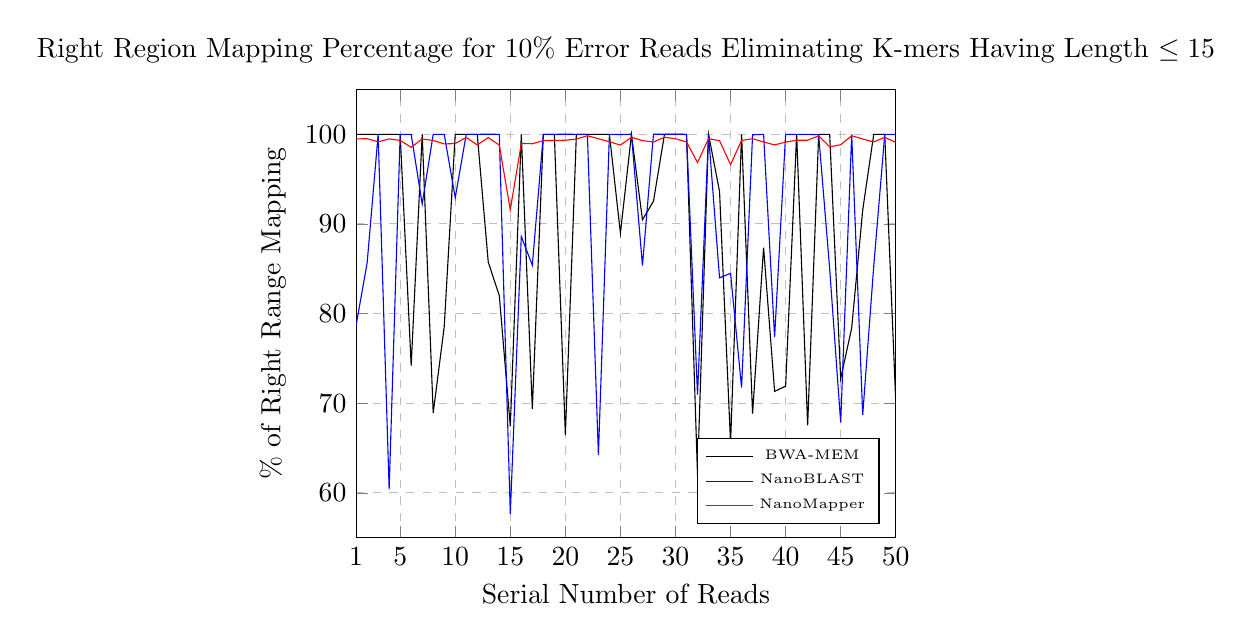
\begin{tikzpicture}
	\begin{axis}[
	title={Right Region Mapping Percentage for 10\% Error Reads Eliminating K-mers Having Length $\leq 15$},
	xlabel={Serial Number of Reads},
	ylabel={\% of Right Range Mapping  },
	xmin=1, xmax=50,
	ymin=55, ymax=105,
	xtick={1,5,10,15,20,25,30,35,40,45,50},
	ytick={60,70,80,90,100},
	legend pos=south east,
	legend style={font=\tiny},
	ymajorgrids=true,
	xmajorgrids=true,
	grid style=dashed,
	]
	
	\addplot[
	color=black,
	mark=dot,
	]
	coordinates {
		( 1 , 99.99 )( 2 , 99.98 )( 3 , 99.98 )( 4 , 99.98 )( 5 , 99.99 )( 6 , 74.19 )( 7 , 99.99 )( 8 , 68.91 )( 9 , 78.53 )( 10 , 99.99 )( 11 , 99.98 )( 12 , 99.98 )( 13 , 85.72 )( 14 , 82.02 )( 15 , 67.43 )( 16 , 99.98 )( 17 , 69.37 )( 18 , 99.98 )( 19 , 99.98 )( 20 , 66.45 )( 21 , 99.98 )( 22 , 99.98 )( 23 , 99.98 )( 24 , 99.98 )( 25 , 88.95 )( 26 , 99.98 )( 27 , 90.46 )( 28 , 92.53 )( 29 , 99.98 )( 30 , 99.98 )( 31 , 99.99 )( 32 , 61.98 )( 33 , 99.99 )( 34 , 93.61 )( 35 , 65.55 )( 36 , 99.98 )( 37 , 68.83 )( 38 , 87.36 )( 39 , 71.32 )( 40 , 71.9 )( 41 , 99.98 )( 42 , 67.52 )( 43 , 99.98 )( 44 , 99.99 )( 45 , 72.76 )( 46 , 78.4 )( 47 , 91.54 )( 48 , 99.98 )( 49 , 99.99 )( 50 , 70.14 )
	};
	\addlegendentry{BWA-MEM}
	\addplot[
	color=blue,
	mark=dot,
	]
	coordinates {
		( 1 , 78.7 )( 2 , 85.64 )( 3 , 99.99 )( 4 , 60.4 )( 5 , 99.99 )( 6 , 99.99 )( 7 , 92.22 )( 8 , 99.99 )( 9 , 99.99 )( 10 , 92.93 )( 11 , 99.99 )( 12 , 99.99 )( 13 , 100.0 )( 14 , 99.99 )( 15 , 57.67 )( 16 , 88.6 )( 17 , 85.39 )( 18 , 99.99 )( 19 , 99.99 )( 20 , 100.0 )( 21 , 99.99 )( 22 , 99.99 )( 23 , 64.24 )( 24 , 99.99 )( 25 , 99.97 )( 26 , 100.0 )( 27 , 85.34 )( 28 , 100.0 )( 29 , 100.0 )( 30 , 100.0 )( 31 , 99.99 )( 32 , 70.96 )( 33 , 99.99 )( 34 , 83.98 )( 35 , 84.5 )( 36 , 71.74 )( 37 , 99.94 )( 38 , 99.99 )( 39 , 77.37 )( 40 , 99.99 )( 41 , 99.99 )( 42 , 99.99 )( 43 , 99.95 )( 44 , 84.98 )( 45 , 67.84 )( 46 , 99.98 )( 47 , 68.7 )( 48 , 85.26 )( 49 , 99.99 )( 50 , 99.99 )
	};
	\addlegendentry{NanoBLAST}
	\addplot[
	color=red,
	mark=dot,
	]
	coordinates {
		( 1 , 99.48 )( 2 , 99.5 )( 3 , 99.16 )( 4 , 99.48 )( 5 , 99.31 )( 6 , 98.54 )( 7 , 99.47 )( 8 , 99.31 )( 9 , 98.92 )( 10 , 98.96 )( 11 , 99.64 )( 12 , 98.81 )( 13 , 99.63 )( 14 , 98.79 )( 15 , 91.57 )( 16 , 98.98 )( 17 , 98.94 )( 18 , 99.29 )( 19 , 99.31 )( 20 , 99.33 )( 21 , 99.47 )( 22 , 99.83 )( 23 , 99.5 )( 24 , 99.16 )( 25 , 98.79 )( 26 , 99.66 )( 27 , 99.29 )( 28 , 99.14 )( 29 , 99.66 )( 30 , 99.5 )( 31 , 99.14 )( 32 , 96.85 )( 33 , 99.5 )( 34 , 99.28 )( 35 , 96.61 )( 36 , 99.31 )( 37 , 99.5 )( 38 , 99.14 )( 39 , 98.81 )( 40 , 99.12 )( 41 , 99.33 )( 42 , 99.33 )( 43 , 99.83 )( 44 , 98.6 )( 45 , 98.83 )( 46 , 99.83 )( 47 , 99.47 )( 48 , 99.14 )( 49 , 99.66 )( 50 , 99.09 )
	};
	\addlegendentry{NanoMapper}
	\end{axis}
	\end{tikzpicture}
	\caption{Percentage of Right Range Mapping Comparison Among Tools After Removing K-mer Having Length Less Than or Equal to 15 For 10\% Noise In Data.} \label{fig:mapComp2}
\end{figure}

\end{document}